\documentclass[./main.tex]{subfiles}

\begin{document}

The purpose of this section is to provide an overview of the system architecture,
on which all the assumptions later on in the document will be based. In
particular, the reference system architecture is represented in figure
\ref{fig:system_architecture}.

\begin{figure}[H]
\centering
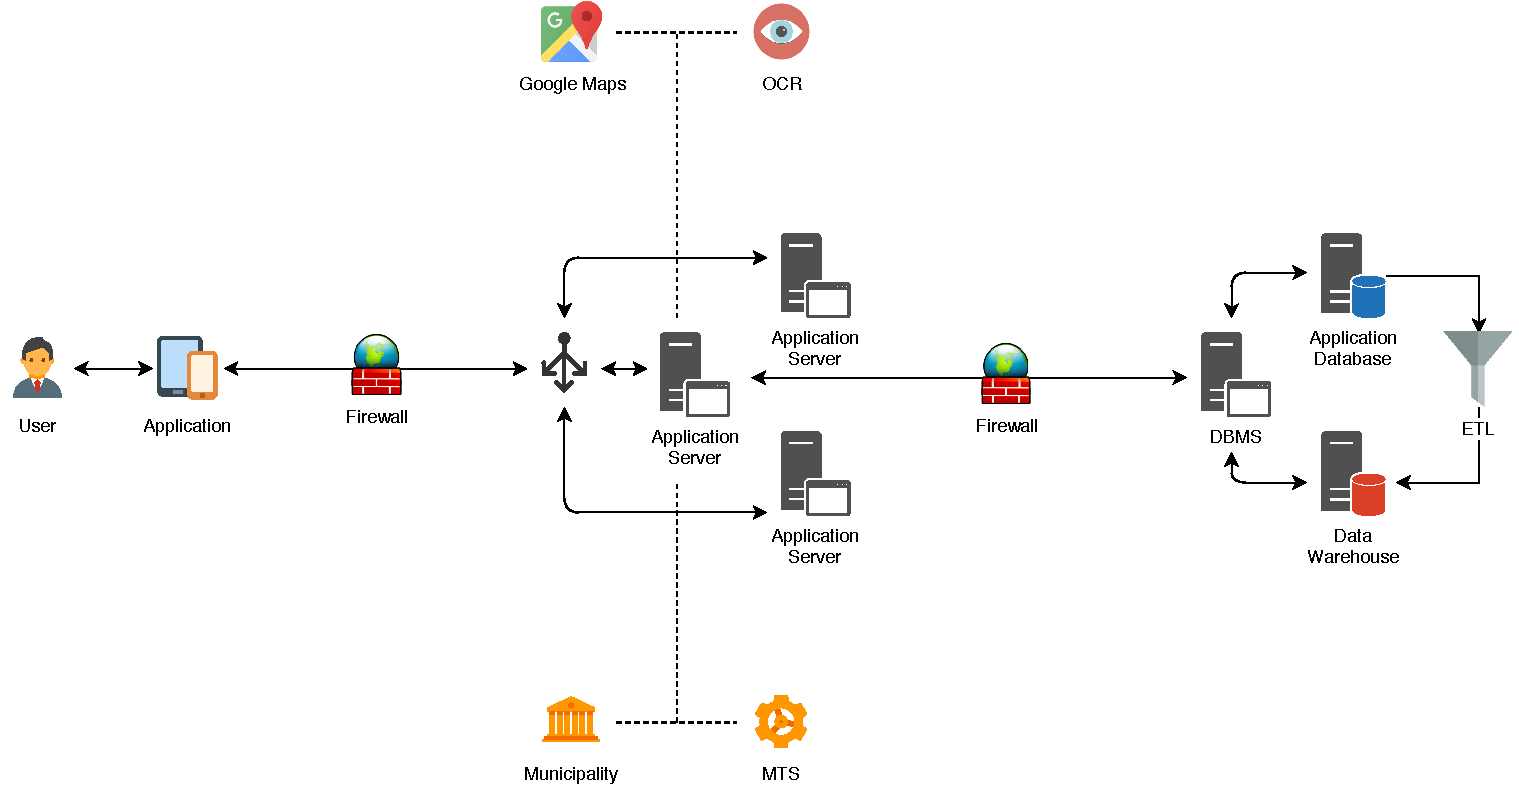
\includegraphics[width=\textwidth]{system_architecture}
\caption{System architecture}
\label{fig:system_architecture}
\end{figure}

The system is built over a 3-tier architecture, where the distinction between the
three layers (presentation, application, data) is evident. Every layer
corresponds to a node that can be developed independently from the others. This
involves scalability and security of the system since every node can be upgraded
without affecting the overall functionality. Moreover, keeping only one channel
for the communication between the user and the application server involves a more
compact architecture. Also, the user-application channel is the only one where a
firewall is placed, to protect the application server from incoming dangers
\medskip\\
Since the application database is centralized, it is possible to replicate the
application server to achieve better performance. To fully take advantage of the
server replication, a load balancer is placed between the user and the
application server. It distributes the workload over the replicated nodes
\medskip\\
The data node consists of the combination of a relational database and a data
warehouse. The database must process a high number of transactions (OLTP policy).
The data warehouse must handle complex queries and data mining over a large
amount of data (OLAP policy). The information flow from the database to the data
warehouse follows an ETL process. The physical implementation of the database and
the data warehouse is not studied in deep since it is not the focus of the
project.

\end{document}